\documentclass{article}
\usepackage[utf8]{inputenc}
\usepackage{amsmath}
\usepackage{graphicx}
\graphicspath{ { images/ } }

% Packages for footnotes in table
\usepackage{footnote}
\makesavenoteenv{tabular}

\title{CS 61B Course Summary}
\author{Matthew Signorotti}
\date{May 2018}

\begin{document}

\maketitle

\section{Data Structures}

\begin{itemize}
    \item \textbf{List}
    \begin{itemize}
        \item \textbf{Linked list}: The simplest list data structure. It features constant-time accessing from and inserting to the front and back of the list. Unfortunately, accessing from and inserting to the middle are linear time.
        \item \textbf{Array list} (resizing array): An array which can be inserted to and deleted from any position. Accessing from any point in the list is constant time, and resizing is amortized (average) constant time if array size can only double or half.
        \begin{itemize}
            \item Suffers when adding to the middle, which requires shifting all the elements to the right by one, or to the front (except in an array-dequeue or other implementation in which the list can actually wrap around to the back of the internal array).
        \end{itemize}
    \end{itemize}
    \item \textbf{Queue}
    \begin{itemize}
        \item A more specific, bare-bones interface which only requires operations to add, remove, and examine elements.
        \item \textbf{Linked list}: See above; it supports adding and removing from not only the front, but also the end.
        \item \textbf{Priority queue}
        \begin{itemize}
            \item \textbf{Minimum heap}: A type of tree data structure which is the most common implementation of a priority queue, and which must obey two properties: completeness and the min-heap property. To be complete, every non-leaf node has the maximum number of children, and the nodes on the bottom level are positioned as much to the ``left'' side of the tree as possible. To obey the min-heap property, every node is greater than or equal to its parents.
            \begin{itemize}
                \item Used in the \texttt{java.util.PriorityQueue} implementation.
            \end{itemize}
            \item \textbf{Maximum heap}: The opposite of a minimum heap. It obeys the same properties, except every node is less than or equal to its parents. Useful if you want to obtain 
            \item What makes the priority queue so great? Why not collect a jumbled set of data and sort it?
            \begin{itemize}
                \item Adding an element is $\Theta(\log N)$, and roughly by that logic, constructing the queue is $\Theta(N\log N)$ --- the same, asymptotically, as adding everything to a collection and then sorting it at the end. In this case, either approach is valid, and you would want to run efficiency tests to determine a strategy.
                \item However, priority queues are truly advantageous for large sets of $N$ elements, of which we only care about a small subset, say $K$ elements:
                \begin{enumerate}
                    \item We only need to store $\Theta(K)$ memory.
                    \item ``Sorting'' through all the information will take $\Theta(N\log K)$ time, not $\Theta(N\log N)$ (the min-heap tree will be maximum $\log K$ height, which is much less than $\log N$).
                \end{enumerate}
            \end{itemize}
        \end{itemize}
        \item The \texttt{ArrayDeque} encountered in CS 61B was an array-implemented queue which could add to both the back and the front of the queue, hence ``double-ended queue.''
    \end{itemize}
    \item \textbf{Stack}
    \begin{itemize}
        \item A queue which is last-in, first-out (LIFO), rather than first-in, first-out (FIFO).
    \end{itemize}
    \item \textbf{Map}
    \begin{itemize}
        \item Hash map
        \begin{itemize}
            \item Chaining (buckets) hash table: Used the most in practice. An array maps \texttt{hashCode \% buckets.length} to linked lists of elements.
            \item Linear probing hash table: No buckets; the internal array contains at most one item, directly. If a spot is filled, linearly ``probe'' the list forward until an open spot is found, or else the operation fails.
            \item Advantage: amortized $\Theta(1)$ (constant-time) addition and retrieval of elements, provided an evenly distributed \texttt{hashCode} function.
            \item The main benefit of hashing over using a primitive list of key-value pairs is not having to do $\Theta(N)$ \texttt{compareTo} computations.
        \end{itemize}
        \item Tree map
        \begin{itemize}
            \item Binary search tree: Very simple implementation which, for a balanced tree, takes $\Theta(\log N)$ for addition and checking for elements. Removal is accomplished by ``promoting'' the minimum element in the right sub-tree, or the maximum element in the left sub-tree.
            \begin{itemize}
                \item Unfortunately, this implementation is less ideal because empirically, after adding and removing from a tree, the tree's height tends toward $\Theta(\sqrt{N})$.
            \end{itemize}
            \item B-trees: Guaranteed to be balanced. A b-tree of magnitude 3, or 2-3 tree, has nodes of up to 2 items and up to 3 children. Objects are inserted into the leaf nodes, and if a node is ``overstuffed'' (exceeds capacity), the tree ``splits'' upward. When splitting, only the middle node, or left-middle if there are two middle nodes, goes upward.
            \begin{figure}[h]
                \centering
                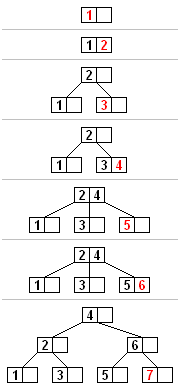
\includegraphics[width=0.25\textwidth]{images/B_tree_insertion_example.png}
                \caption{Inserting into a left-leaning b-tree of magnitude 3 (2-3 tree)}
                \label{fig:my_label}
            \end{figure}
            \item (Left-leaning) Red-black trees: Unlike b-trees, these perform well and can be searched just like a binary search tree. To construct one, start with a b-tree. Then, for every node with multiple items, keep the rightmost item as the root node, and each item to the left becomes the left child of the current node.
        \end{itemize}
        \item Tries
        \begin{itemize}
            \item A tree in which each node represents a character or digit of a greater expression. Stopping at a certain node tells whether the sequence of characters from the root to that point is contained in the map. In most trie implementations, the character each node represents is the character represented by the mapping to that node in its parent's \texttt{children} map/array.
            \item Ternary search trie: A less conventional idea in which nodes of equivalent depth and with the same parent as an existing node are added to that node's \texttt{left} or \texttt{right} attribute.
            \begin{figure}[h]
                \centering
                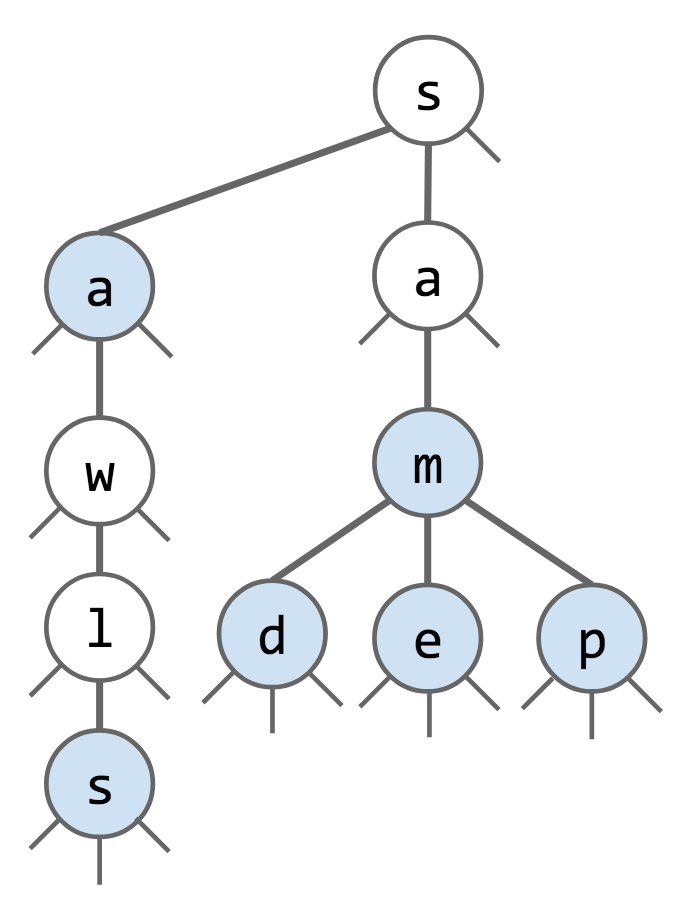
\includegraphics[width=0.35\textwidth]{images/TernarySearchTrie.png}
                \caption{Ternary search trie after inserting ``a'', ``awls'', ``sam'', ``sad'', ``sap'', and ``same''}
                \label{fig:my_label}
            \end{figure}
            \item Particularly effective to retrieve items which share a prefix, or for digit-by-digit problems such as radix sort. Used primarily for its rapid prefix matching.
            \item Highly space efficient, more so than a hash set, but potentially less time efficient to retrieve items with non-constant time \texttt{hashCode} functions.
            \item Unlike other abstract data types, lacks a widely used implementation in \texttt{java.util}.
        \end{itemize}
    \end{itemize}
    \item \textbf{Set}
    \begin{itemize}
        \item Hash sets: See above.
        \item Tree sets: See above.
        \item Tries: See above.
        \item Any map implementation can be reduced to a set implementation.
    \end{itemize}
    \item \textbf{Graph}
    \begin{figure}[h]
        \centering
        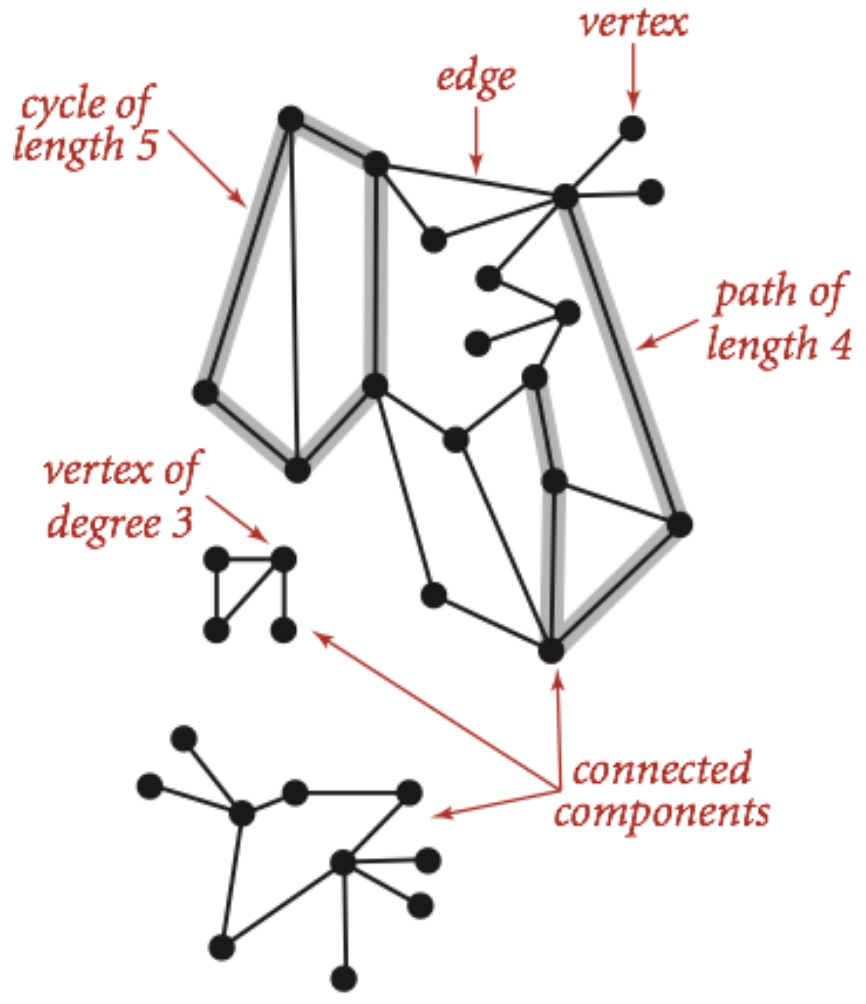
\includegraphics[width=0.4\textwidth]{images/Graphs.png}
        \caption{Graph terminology}
        \label{fig:my_label}
    \end{figure}
    \begin{itemize}
        \item Vertices typically have numbers, and are looked up with something like a map from strings to integers.
        \item Adjacency matrix (initial attempt): Two-dimensional matrix telling whether two vertices are connected. Not as great: $\Theta(V^2)$ space and $\Theta(V)$ time to look up adjacent vertices.
        \item Edge set: Hash set of pairs of integers representing connections.
        \item Adjacency list: A map or array records a list of ``children'' for every node.
        \begin{itemize}
            \item A similar representation was used in Project 3, except we went further by creating node objects which contain sets of children.
        \end{itemize}
    \end{itemize}
    \item \textbf{Disjoint set}
    \begin{itemize}
        \item Support two operations: \texttt{connect} and \texttt{isConnected}.
        \item How we designed the data structure:
        \begin{itemize}
            \item Attempt \#1, \texttt{QuickFindDS}: Optimize \texttt{isConnected}. Simply map item numbers to an integer representing the number of the set each is part of. This has constant time \texttt{isConnected}, but \texttt{connect} is a different story.
            \item Attempt \#2, \texttt{QuickUnionDS}: Array-based trees (array-based since we need to find any node quickly) represent each set. Connect trees to connect elements; trace items to their roots to see if they are connected.
            \item Attempt \#3, \texttt{WeightedQuickUnionDS}: Same as attempt \# 2, except to connect sets, always connect the tree of fewer nodes to the root of the other one.
            \item Path compression: A very efficient optimization. Whenever we call \texttt{connect}, we call a \texttt{find} helper function on both arguments to find the roots of their respective trees. The path compression optimization attaches each parent node of \texttt{find}'s argument directly to the root. \texttt{find} will initially still take logarithmic time, but called again on the same argument, it will take constant time.
        \end{itemize}
    \end{itemize}
\end{itemize}

\section{Algorithms}

\subsection*{Tree (and Graph) Traversals}

\begin{figure}[h]
    \centering
    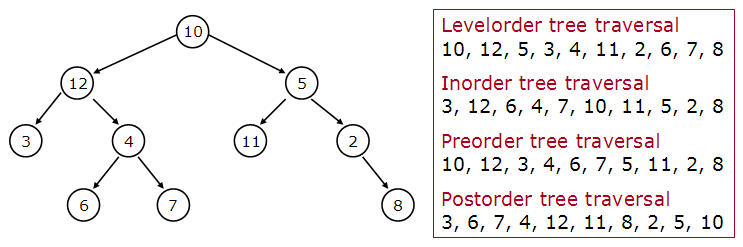
\includegraphics[width=0.8\textwidth]{images/TreeTraversals.png}
    \caption{The three depth-first tree traversals}
    \label{fig:my_label}
\end{figure}

\begin{itemize}
    \item Depth-first traversals
    \begin{itemize}
        \item Implemented recursively or with a stack data structure, as used below.
        \item Pre-order traversal: Add or print the current node, and the children to the stack, and retrieve the next node from the stack.
        \item In-order traversal: Add the left child to the stack, add or print the current node, and then add the right child to the stack.
        \item Post-order traversal: Add the children to the stack and then add or print the current node.
    \end{itemize}
    \item Breadth-first traversal: Use a queue to choose the next node. Add or print the current node, add all its children to the queue, and dequeue the next item.
    \item The same traversals can be extended to graph algorithms. For graphs, which have loops, make sure to mark each node so as not to reach the same node multiple times and encounter an infinite loop.
\end{itemize}

\subsection*{Graph Algorithms}

\begin{itemize}
    \item \textbf{Search algorithms}
    \begin{itemize}
        \item $\Theta(V)$ space
        \item Breadth-first search: See above. $\Theta(V + E)$ time.
        \item Depth-first search: See above. $\Theta(V + E)$ time.
        \item Dijkstra's algorithm: Used to find shortest paths to a point or every point from a source. Using a priority queue, expand the graph vertex by vertex, choosing vertices of minimum distance from the source. All edge weights should have the same sign, i.e. non-negative. Implemented with a min-heap, is $O(E\log V)$.
        \item A* search algorithm: Same as Dijkstra's, except vertices are ordered by some estimate heuristic representing the minimum amount of work to reach the target. Used in artificial intelligence, Google Maps; highly efficient to find the shortest path from one node to another. Best runtime, but no clear asymptotic complexity without knowing the heuristic.
    \end{itemize}
    \item \textbf{Minimum spanning tree}
    \begin{itemize}
        \item Cut property: For all edges connecting two sets of vertices, the minimum spanning tree will contain just one of those edges, and it will be the smallest one.
        \item Prim's algorithm: Starting with a tree of just one node, create a priority queue to sort edges by weight. Adding edges touched by the tree, and using a disjoint set to prevent cycles, add $N - 1$ edges.
        \item Kruskall's alogirhtm: Sort the edges into a priority queue. Add $N - 1$ edges which, according to a disjoint set, do not create a cycle.
        \item Maximum spanning tree: Multiply the weights by $-1$; run either algorithm.
    \end{itemize}
    \item \textbf{Topological sorting}: Generating a valid ordering of vertices in which, for each vertex, its ``parents'' are before it in the ordering. This is achieved by a reverse post-order, or simply the post-order traversal of a list, reversed. A breadth-first search also works if the graph has only one source node.
\end{itemize}

\subsection*{Sorting}

\begin{center}
    \begin{tabular}{c || c c c} 
        & \textbf{Time} & \textbf{Memory} & \textbf{Usage} \\ [0.5ex]
        \hline\hline
        Quick sort & $\Theta(N\log N)$ to $\Theta(N^2)$ & $\Theta(\log N)$ & Fastest, but unstable \\
        Merge sort & $\Theta(N\log N)$ & $\Theta(N)$\footnote{Common implementations do not sort in place, leading to $\Theta(N)$ memory.} & Best stable sort \\
        Heap sort & $\Theta(N$ to $N\log N)$\footnote{$\Theta(N)$ is possible for an array of all duplicates.} & $\Theta(1)$ & Bad caching (hardware) \\
        Insertion sort & $\Theta(N + K)$\footnote{$K$ inversions (pairs of items in which the left is greater than the right).} to $\Theta(N^2)$ & $\Theta(1)$ & Almost-sorted arrays \\
        Radix sort & $\Theta(L(N + R))$ &  & Bounded-length data \\ [1ex]
    \end{tabular}
\end{center}

\subsubsection*{Comparison Sorts}

\begin{itemize}
    \item \textbf{Quick sort}: The best performance empirically. Pick an element to partition around, preferably randomly so that the algorithm can't be ``broken,'' and throw everything either right or left of it. Then sort the left and right sides of that element.
    \item \textbf{Merge sort}: Sort two halves, then merge them into one whole. Alternatively, can be implemented iteratively from the ``bottom up'' --- sort every two elements, then every four, etc.
    \item \textbf{Heap sort}: From right to left, ``heapify'' the input array (this $\Theta(N)$ bottom-up approach beats $\Theta(N\log N)$ top-down, due to some fancy math --- see Discussion 13 for a proof). Then empty the heap, reinserting the items at the end. Despite its great asymptotic complexity, rarely used due to its bad caching performance.
    \item \textbf{Insertion sort}: For each element which is less than the element next to it, swap it leftward until it is greater than the adjacent element.
    \item \textbf{Selection sort}: \underline{Avoid!} Has $\Theta(N^2)$ runtime. For each index, it finds the minimum element left of that index, and swaps it into the position.
\end{itemize}

Comparison sorts such as quick sort and merge sort are believed to have achieved \textit{ideal} asymptotic runtime for a sort which uses \texttt{compareTo} to order items. This is because for $N$ items, the sorting problem can be reduced to a decision tree with $N!$ leaf nodes, each representing an arrangement of the $N$ objects, and a height of $\Theta(\log N!)$. (This assumes the tree has a constant branching factor throughout, which is fairly intuitive, but not entirely justified.) The number of decisions, $\Theta(\log N!)$, is a runtime equivalent to $\Theta(N \log N)$ because of the following proof:
$$\log N! = \log N + \log (N - 1) + \cdots + \log 1 \longrightarrow N\log N \in \Omega(\log N!)$$
\vspace{-6mm}
$$N! > (N/2)^{N/2} \longrightarrow \log N! > \log (N/2)^{N/2} \longrightarrow \log N! \in \Omega(N\log N)$$
$$\log N! \in \Theta(N \log N)$$

\subsubsection*{Radix Sorts}

The above ``ideal'' runtime is for sorts based on comparing items, but could there be a different type of sort with better runtime?

\begin{itemize}
    \item \textbf{Counting sort} (subroutine for radix sort): Count the frequencies of each of $R$ digits in the input. Use these frequencies to generate starting indices to place objects in the output array. Iterate through the input array and place each item at its starting index in the output array, updating the starting index.
    \item \textbf{Radix sort}: For each digit position in the input data, perform a counting sort. LSD (least significant digit) sort starts with the least significant, typically rightmost, digit. MSD sort does the opposite, and it also has to subdivide/group the subproblems by digit in the most recently sorted index.
    \begin{itemize}
        \item Runtime $\Theta(L(N + R))$ is proportional to the number of digits $L$, the number of counting sorts required. Each counting sort iterates over $N$ indices and must create a frequency arrays of length $R$, to accommodate every possible digit.
        \item Performs best only if $L$ is bounded by a constant. For instance, integers or fixed-length strings have a maximum size.
    \end{itemize}
\end{itemize}

\end{document}
